\documentclass[a4paper]{article}
\usepackage[margin=1cm]{geometry}
\usepackage{amsmath, amssymb}
\usepackage{graphicx}
\usepackage{tikz}
\usetikzlibrary{arrows.meta}
\pagestyle{empty}

\definecolor{c0}{HTML}{E53935}
\definecolor{c1}{HTML}{1E88E5}
\definecolor{c2}{HTML}{43A047}
\definecolor{c3}{HTML}{FB8C00}
\definecolor{c4}{HTML}{8E24AA}
\definecolor{c5}{HTML}{00ACC1}
\definecolor{c6}{HTML}{F4511E}
\definecolor{c7}{HTML}{3949AB}
\definecolor{c8}{HTML}{7CB342}
\definecolor{c9}{HTML}{C2185B}
\definecolor{c10}{HTML}{FF7043}
\definecolor{c11}{HTML}{26A69A}
\definecolor{c12}{HTML}{5C6BC0}
\definecolor{c13}{HTML}{FFCA28}
\definecolor{c14}{HTML}{AB47BC}

\begin{document}

\begin{center}
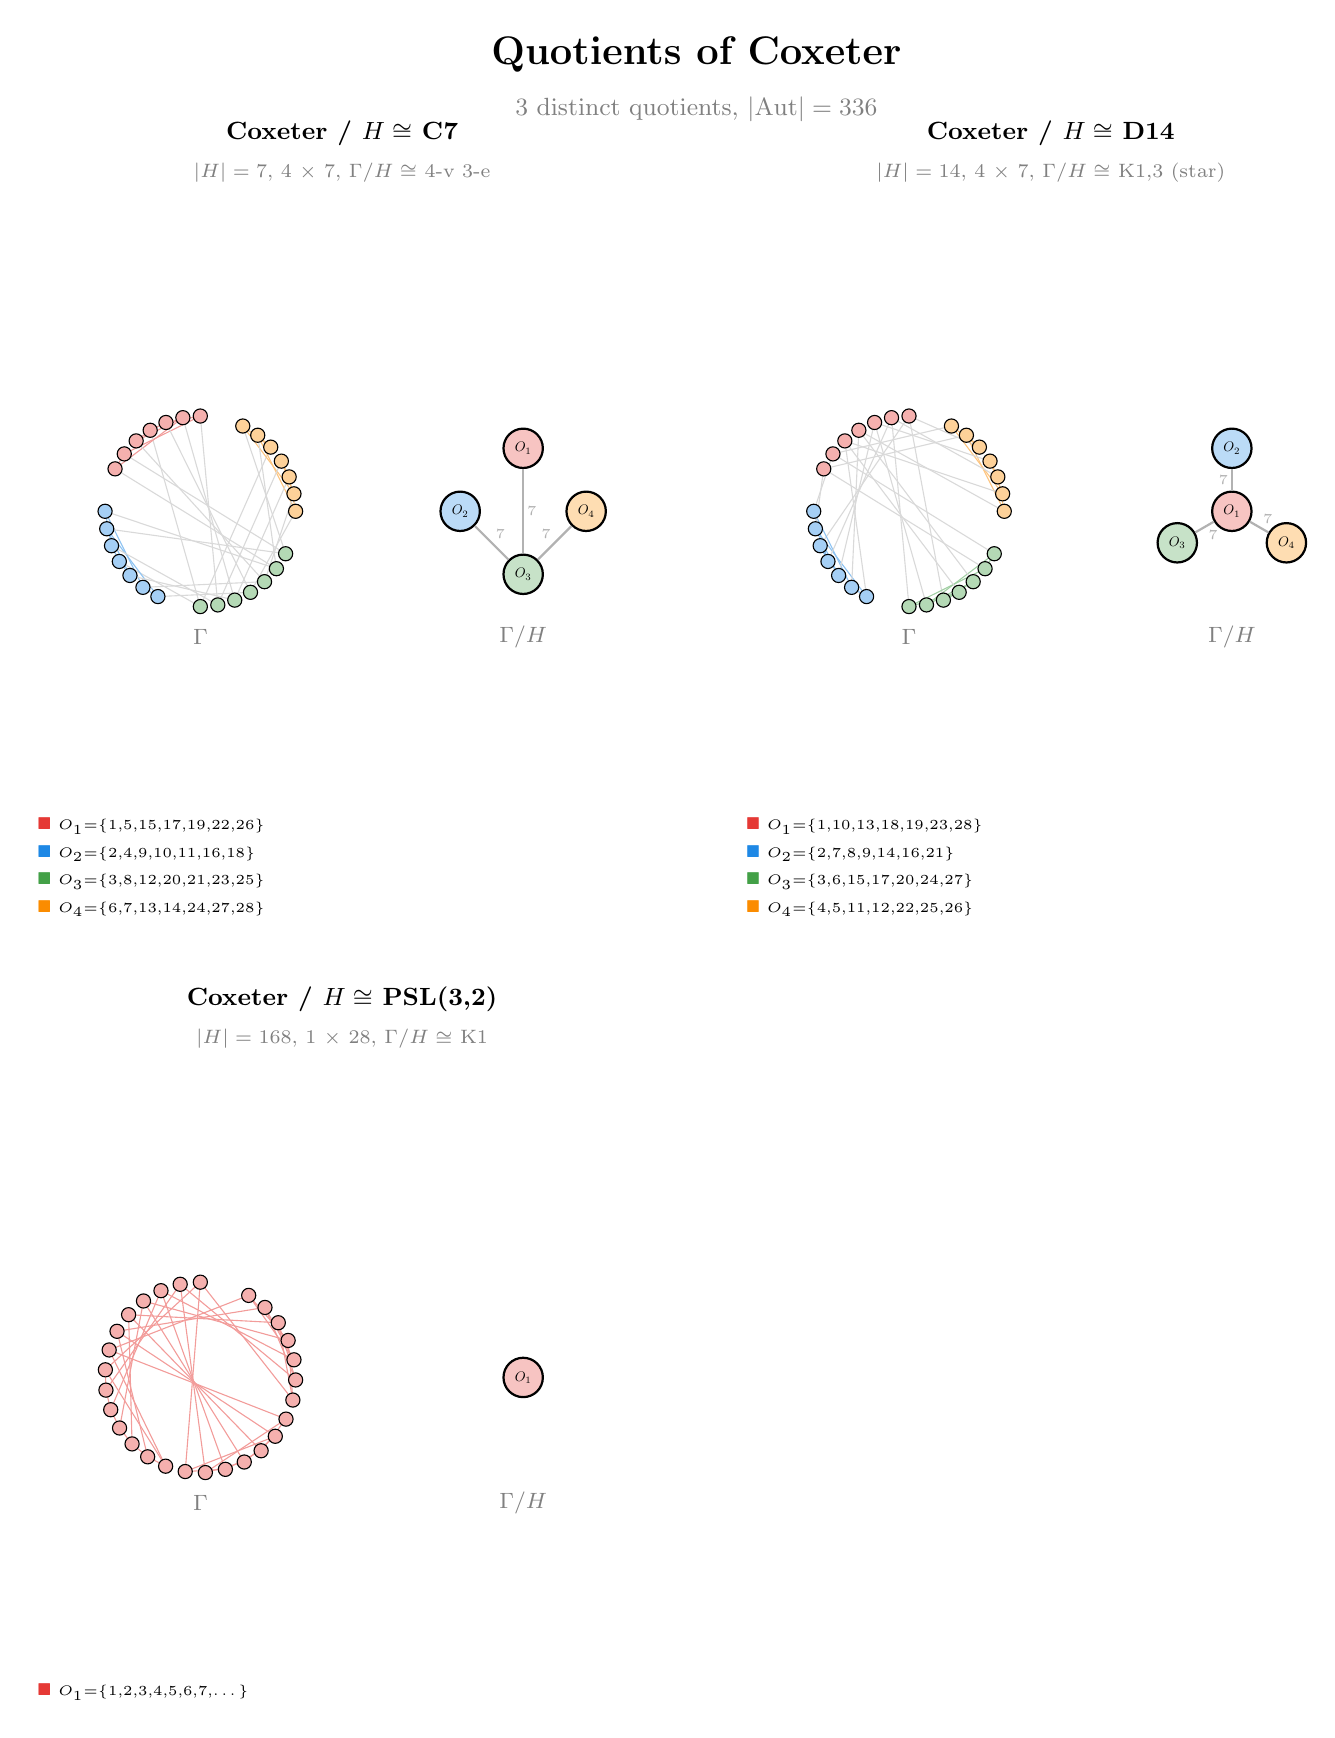
\begin{tikzpicture}[
  ov/.style={circle, draw, semithick, minimum size=3.5mm, inner sep=0pt},
  ovs/.style={circle, draw, thin, minimum size=1.8mm, inner sep=0pt},
  qv/.style={circle, draw, thick, minimum size=5mm, inner sep=0pt},
  cardtitle/.style={font=\small\bfseries},
  cardsub/.style={font=\scriptsize, text=gray},
  glabel/.style={font=\footnotesize, text=gray},
]
\node[font=\Large\bfseries] at (0, 11.5) {Quotients of Coxeter};
\node[font=\small, text=gray] at (0, 10.8) {3 distinct quotients, $|\mathrm{Aut}|=336$};

% Card 1: H=C7
\node[cardtitle] at (-4.50,10.50) {Coxeter / $H \cong$ C7};
\node[cardsub] at (-4.50,10.00) {$|H|=7$, 4 $\times$ 7, $\Gamma/H \cong$ 4-v 3-e};
\draw[gray!30, thin] (-6.300,6.910) -- (-6.078,4.511);
\draw[c0!50, thin] (-6.300,6.910) -- (-6.737,6.828);
\draw[c0!50, thin] (-6.300,6.910) -- (-7.266,6.429);
\draw[c1!50, thin] (-7.510,5.700) -- (-7.428,5.263);
\draw[c1!50, thin] (-7.510,5.700) -- (-7.029,4.734);
\draw[gray!30, thin] (-7.510,5.700) -- (-5.334,4.971);
\draw[gray!30, thin] (-6.300,4.490) -- (-7.329,5.063);
\draw[gray!30, thin] (-6.300,4.490) -- (-6.937,6.729);
\draw[gray!30, thin] (-6.300,4.490) -- (-5.406,6.515);
\draw[c1!50, thin] (-7.489,5.478) -- (-7.194,4.885);
\draw[c1!50, thin] (-7.489,5.478) -- (-6.839,4.617);
\draw[gray!30, thin] (-7.489,5.478) -- (-5.217,5.161);
\draw[gray!30, thin] (-6.522,6.889) -- (-5.863,4.572);
\draw[c0!50, thin] (-6.522,6.889) -- (-7.115,6.594);
\draw[c0!50, thin] (-6.522,6.889) -- (-7.383,6.239);
\draw[c3!50, thin] (-5.090,5.700) -- (-5.172,6.137);
\draw[gray!30, thin] (-5.090,5.700) -- (-5.663,4.671);
\draw[c3!50, thin] (-5.090,5.700) -- (-5.571,6.666);
\draw[c3!50, thin] (-5.111,5.922) -- (-5.271,6.337);
\draw[gray!30, thin] (-5.111,5.922) -- (-5.485,4.806);
\draw[c3!50, thin] (-5.111,5.922) -- (-5.761,6.783);
\draw[gray!30, thin] (-6.078,4.511) -- (-7.428,5.263);
\draw[gray!30, thin] (-6.078,4.511) -- (-5.271,6.337);
\draw[c1!50, thin] (-7.428,5.263) -- (-7.329,5.063);
\draw[c1!50, thin] (-7.329,5.063) -- (-7.194,4.885);
\draw[gray!30, thin] (-7.194,4.885) -- (-5.863,4.572);
\draw[gray!30, thin] (-5.863,4.572) -- (-5.172,6.137);
\draw[c3!50, thin] (-5.172,6.137) -- (-5.271,6.337);
\draw[c0!50, thin] (-6.737,6.828) -- (-6.937,6.729);
\draw[gray!30, thin] (-6.737,6.828) -- (-5.663,4.671);
\draw[c1!50, thin] (-7.029,4.734) -- (-6.839,4.617);
\draw[gray!30, thin] (-7.029,4.734) -- (-5.485,4.806);
\draw[c0!50, thin] (-6.937,6.729) -- (-7.115,6.594);
\draw[gray!30, thin] (-6.839,4.617) -- (-5.663,4.671);
\draw[gray!30, thin] (-7.115,6.594) -- (-5.485,4.806);
\draw[gray!30, thin] (-7.266,6.429) -- (-5.217,5.161);
\draw[c0!50, thin] (-7.266,6.429) -- (-7.383,6.239);
\draw[gray!30, thin] (-5.334,4.971) -- (-7.383,6.239);
\draw[gray!30, thin] (-5.334,4.971) -- (-5.571,6.666);
\draw[c3!50, thin] (-5.406,6.515) -- (-5.571,6.666);
\draw[c3!50, thin] (-5.406,6.515) -- (-5.761,6.783);
\draw[gray!30, thin] (-5.217,5.161) -- (-5.761,6.783);
\node[ovs, fill=c0!40] at (-6.300,6.910) {};
\node[ovs, fill=c1!40] at (-7.510,5.700) {};
\node[ovs, fill=c2!40] at (-6.300,4.490) {};
\node[ovs, fill=c1!40] at (-7.489,5.478) {};
\node[ovs, fill=c0!40] at (-6.522,6.889) {};
\node[ovs, fill=c3!40] at (-5.090,5.700) {};
\node[ovs, fill=c3!40] at (-5.111,5.922) {};
\node[ovs, fill=c2!40] at (-6.078,4.511) {};
\node[ovs, fill=c1!40] at (-7.428,5.263) {};
\node[ovs, fill=c1!40] at (-7.329,5.063) {};
\node[ovs, fill=c1!40] at (-7.194,4.885) {};
\node[ovs, fill=c2!40] at (-5.863,4.572) {};
\node[ovs, fill=c3!40] at (-5.172,6.137) {};
\node[ovs, fill=c3!40] at (-5.271,6.337) {};
\node[ovs, fill=c0!40] at (-6.737,6.828) {};
\node[ovs, fill=c1!40] at (-7.029,4.734) {};
\node[ovs, fill=c0!40] at (-6.937,6.729) {};
\node[ovs, fill=c1!40] at (-6.839,4.617) {};
\node[ovs, fill=c0!40] at (-7.115,6.594) {};
\node[ovs, fill=c2!40] at (-5.663,4.671) {};
\node[ovs, fill=c2!40] at (-5.485,4.806) {};
\node[ovs, fill=c0!40] at (-7.266,6.429) {};
\node[ovs, fill=c2!40] at (-5.334,4.971) {};
\node[ovs, fill=c3!40] at (-5.406,6.515) {};
\node[ovs, fill=c2!40] at (-5.217,5.161) {};
\node[ovs, fill=c0!40] at (-7.383,6.239) {};
\node[ovs, fill=c3!40] at (-5.571,6.666) {};
\node[ovs, fill=c3!40] at (-5.761,6.783) {};
\node[glabel] at (-6.30,4.10) {$\Gamma$};
\node[qv, fill=c0!30] (c0o0) at (-2.200,6.500) {\scalebox{0.5}{$O_{1}$}};
\node[qv, fill=c1!30] (c0o1) at (-3.000,5.700) {\scalebox{0.5}{$O_{2}$}};
\node[qv, fill=c2!30] (c0o2) at (-2.200,4.900) {\scalebox{0.5}{$O_{3}$}};
\node[qv, fill=c3!30] (c0o3) at (-1.400,5.700) {\scalebox{0.5}{$O_{4}$}};
\draw[gray!60, thick] (c0o0) -- node[font=\tiny, auto, inner sep=1pt] {7} (c0o2);
\draw[gray!60, thick] (c0o1) -- node[font=\tiny, auto, inner sep=1pt] {7} (c0o2);
\draw[gray!60, thick] (c0o2) -- node[font=\tiny, auto, inner sep=1pt] {7} (c0o3);
\node[glabel] at (-2.20,4.10) {$\Gamma/H$};
\node[anchor=west, font=\tiny] at (-8.50,1.70) {\textcolor{c0}{$\blacksquare$} $O_{1}$=\{1,5,15,17,19,22,26\}};
\node[anchor=west, font=\tiny] at (-8.50,1.35) {\textcolor{c1}{$\blacksquare$} $O_{2}$=\{2,4,9,10,11,16,18\}};
\node[anchor=west, font=\tiny] at (-8.50,1.00) {\textcolor{c2}{$\blacksquare$} $O_{3}$=\{3,8,12,20,21,23,25\}};
\node[anchor=west, font=\tiny] at (-8.50,0.65) {\textcolor{c3}{$\blacksquare$} $O_{4}$=\{6,7,13,14,24,27,28\}};

% Card 2: H=D14
\node[cardtitle] at (4.50,10.50) {Coxeter / $H \cong$ D14};
\node[cardsub] at (4.50,10.00) {$|H|=14$, 4 $\times$ 7, $\Gamma/H \cong$ K1,3 (star)};
\draw[gray!30, thin] (2.700,6.910) -- (1.572,5.263);
\draw[gray!30, thin] (2.700,6.910) -- (3.137,4.572);
\draw[gray!30, thin] (2.700,6.910) -- (3.594,6.515);
\draw[c1!50, thin] (1.490,5.700) -- (1.671,5.063);
\draw[c1!50, thin] (1.490,5.700) -- (1.971,4.734);
\draw[gray!30, thin] (1.490,5.700) -- (1.734,6.429);
\draw[gray!30, thin] (2.700,4.490) -- (2.478,6.889);
\draw[c2!50, thin] (2.700,4.490) -- (3.337,4.671);
\draw[c2!50, thin] (2.700,4.490) -- (3.666,4.971);
\draw[c3!50, thin] (3.910,5.700) -- (3.828,6.137);
\draw[gray!30, thin] (3.910,5.700) -- (2.063,6.729);
\draw[c3!50, thin] (3.910,5.700) -- (3.429,6.666);
\draw[c3!50, thin] (3.889,5.922) -- (3.729,6.337);
\draw[gray!30, thin] (3.889,5.922) -- (1.885,6.594);
\draw[c3!50, thin] (3.889,5.922) -- (3.239,6.783);
\draw[gray!30, thin] (2.922,4.511) -- (2.263,6.828);
\draw[c2!50, thin] (2.922,4.511) -- (3.515,4.806);
\draw[c2!50, thin] (2.922,4.511) -- (3.783,5.161);
\draw[c1!50, thin] (1.511,5.478) -- (1.806,4.885);
\draw[c1!50, thin] (1.511,5.478) -- (2.161,4.617);
\draw[gray!30, thin] (1.511,5.478) -- (1.617,6.239);
\draw[c1!50, thin] (1.572,5.263) -- (1.671,5.063);
\draw[c1!50, thin] (1.572,5.263) -- (1.806,4.885);
\draw[gray!30, thin] (1.671,5.063) -- (2.478,6.889);
\draw[gray!30, thin] (2.478,6.889) -- (3.828,6.137);
\draw[c3!50, thin] (3.828,6.137) -- (3.729,6.337);
\draw[gray!30, thin] (3.729,6.337) -- (2.263,6.828);
\draw[gray!30, thin] (2.263,6.828) -- (1.806,4.885);
\draw[c2!50, thin] (3.137,4.572) -- (3.337,4.671);
\draw[c2!50, thin] (3.137,4.572) -- (3.515,4.806);
\draw[gray!30, thin] (1.971,4.734) -- (2.063,6.729);
\draw[c1!50, thin] (1.971,4.734) -- (2.161,4.617);
\draw[gray!30, thin] (3.337,4.671) -- (1.885,6.594);
\draw[gray!30, thin] (2.063,6.729) -- (3.515,4.806);
\draw[gray!30, thin] (1.885,6.594) -- (2.161,4.617);
\draw[c3!50, thin] (3.594,6.515) -- (3.429,6.666);
\draw[c3!50, thin] (3.594,6.515) -- (3.239,6.783);
\draw[gray!30, thin] (1.734,6.429) -- (3.239,6.783);
\draw[gray!30, thin] (1.734,6.429) -- (3.783,5.161);
\draw[c2!50, thin] (3.666,4.971) -- (3.783,5.161);
\draw[gray!30, thin] (3.666,4.971) -- (1.617,6.239);
\draw[gray!30, thin] (3.429,6.666) -- (1.617,6.239);
\node[ovs, fill=c0!40] at (2.700,6.910) {};
\node[ovs, fill=c1!40] at (1.490,5.700) {};
\node[ovs, fill=c2!40] at (2.700,4.490) {};
\node[ovs, fill=c3!40] at (3.910,5.700) {};
\node[ovs, fill=c3!40] at (3.889,5.922) {};
\node[ovs, fill=c2!40] at (2.922,4.511) {};
\node[ovs, fill=c1!40] at (1.511,5.478) {};
\node[ovs, fill=c1!40] at (1.572,5.263) {};
\node[ovs, fill=c1!40] at (1.671,5.063) {};
\node[ovs, fill=c0!40] at (2.478,6.889) {};
\node[ovs, fill=c3!40] at (3.828,6.137) {};
\node[ovs, fill=c3!40] at (3.729,6.337) {};
\node[ovs, fill=c0!40] at (2.263,6.828) {};
\node[ovs, fill=c1!40] at (1.806,4.885) {};
\node[ovs, fill=c2!40] at (3.137,4.572) {};
\node[ovs, fill=c1!40] at (1.971,4.734) {};
\node[ovs, fill=c2!40] at (3.337,4.671) {};
\node[ovs, fill=c0!40] at (2.063,6.729) {};
\node[ovs, fill=c0!40] at (1.885,6.594) {};
\node[ovs, fill=c2!40] at (3.515,4.806) {};
\node[ovs, fill=c1!40] at (2.161,4.617) {};
\node[ovs, fill=c3!40] at (3.594,6.515) {};
\node[ovs, fill=c0!40] at (1.734,6.429) {};
\node[ovs, fill=c2!40] at (3.666,4.971) {};
\node[ovs, fill=c3!40] at (3.429,6.666) {};
\node[ovs, fill=c3!40] at (3.239,6.783) {};
\node[ovs, fill=c2!40] at (3.783,5.161) {};
\node[ovs, fill=c0!40] at (1.617,6.239) {};
\node[glabel] at (2.70,4.10) {$\Gamma$};
\node[qv, fill=c0!30] (c1o0) at (6.800,5.700) {\scalebox{0.5}{$O_{1}$}};
\node[qv, fill=c1!30] (c1o1) at (6.800,6.500) {\scalebox{0.5}{$O_{2}$}};
\node[qv, fill=c2!30] (c1o2) at (6.107,5.300) {\scalebox{0.5}{$O_{3}$}};
\node[qv, fill=c3!30] (c1o3) at (7.493,5.300) {\scalebox{0.5}{$O_{4}$}};
\draw[gray!60, thick] (c1o0) -- node[font=\tiny, auto, inner sep=1pt] {7} (c1o1);
\draw[gray!60, thick] (c1o0) -- node[font=\tiny, auto, inner sep=1pt] {7} (c1o2);
\draw[gray!60, thick] (c1o0) -- node[font=\tiny, auto, inner sep=1pt] {7} (c1o3);
\node[glabel] at (6.80,4.10) {$\Gamma/H$};
\node[anchor=west, font=\tiny] at (0.50,1.70) {\textcolor{c0}{$\blacksquare$} $O_{1}$=\{1,10,13,18,19,23,28\}};
\node[anchor=west, font=\tiny] at (0.50,1.35) {\textcolor{c1}{$\blacksquare$} $O_{2}$=\{2,7,8,9,14,16,21\}};
\node[anchor=west, font=\tiny] at (0.50,1.00) {\textcolor{c2}{$\blacksquare$} $O_{3}$=\{3,6,15,17,20,24,27\}};
\node[anchor=west, font=\tiny] at (0.50,0.65) {\textcolor{c3}{$\blacksquare$} $O_{4}$=\{4,5,11,12,22,25,26\}};

% Card 3: H=PSL(3,2)
\node[cardtitle] at (-4.50,-0.50) {Coxeter / $H \cong$ PSL(3,2)};
\node[cardsub] at (-4.50,-1.00) {$|H|=168$, 1 $\times$ 28, $\Gamma/H \cong$ K1};
\draw[c0!50, thin] (-6.300,-4.090) -- (-7.506,-5.203);
\draw[c0!50, thin] (-6.300,-4.090) -- (-6.492,-6.495);
\draw[c0!50, thin] (-6.300,-4.090) -- (-5.125,-5.587);
\draw[c0!50, thin] (-6.556,-4.117) -- (-7.499,-5.461);
\draw[c0!50, thin] (-6.556,-4.117) -- (-6.236,-6.508);
\draw[c0!50, thin] (-6.556,-4.117) -- (-5.090,-5.332);
\draw[c0!50, thin] (-6.800,-4.198) -- (-7.438,-5.710);
\draw[c0!50, thin] (-6.800,-4.198) -- (-5.982,-6.467);
\draw[c0!50, thin] (-6.800,-4.198) -- (-5.111,-5.076);
\draw[c0!50, thin] (-7.022,-4.329) -- (-7.326,-5.942);
\draw[c0!50, thin] (-7.022,-4.329) -- (-5.742,-6.374);
\draw[c0!50, thin] (-7.022,-4.329) -- (-5.185,-4.830);
\draw[c0!50, thin] (-7.211,-4.503) -- (-7.167,-6.144);
\draw[c0!50, thin] (-7.211,-4.503) -- (-5.528,-6.231);
\draw[c0!50, thin] (-7.211,-4.503) -- (-5.310,-4.605);
\draw[c0!50, thin] (-7.358,-4.714) -- (-6.969,-6.308);
\draw[c0!50, thin] (-7.358,-4.714) -- (-5.348,-6.047);
\draw[c0!50, thin] (-7.358,-4.714) -- (-5.479,-4.411);
\draw[c0!50, thin] (-7.458,-4.951) -- (-6.741,-6.427);
\draw[c0!50, thin] (-7.458,-4.951) -- (-5.212,-5.829);
\draw[c0!50, thin] (-7.458,-4.951) -- (-5.686,-4.258);
\draw[c0!50, thin] (-7.506,-5.203) -- (-7.499,-5.461);
\draw[c0!50, thin] (-7.506,-5.203) -- (-6.741,-6.427);
\draw[c0!50, thin] (-7.499,-5.461) -- (-7.438,-5.710);
\draw[c0!50, thin] (-7.438,-5.710) -- (-7.326,-5.942);
\draw[c0!50, thin] (-7.326,-5.942) -- (-7.167,-6.144);
\draw[c0!50, thin] (-7.167,-6.144) -- (-6.969,-6.308);
\draw[c0!50, thin] (-6.969,-6.308) -- (-6.741,-6.427);
\draw[c0!50, thin] (-6.492,-6.495) -- (-5.982,-6.467);
\draw[c0!50, thin] (-6.492,-6.495) -- (-5.348,-6.047);
\draw[c0!50, thin] (-6.236,-6.508) -- (-5.742,-6.374);
\draw[c0!50, thin] (-6.236,-6.508) -- (-5.212,-5.829);
\draw[c0!50, thin] (-5.982,-6.467) -- (-5.528,-6.231);
\draw[c0!50, thin] (-5.742,-6.374) -- (-5.348,-6.047);
\draw[c0!50, thin] (-5.528,-6.231) -- (-5.212,-5.829);
\draw[c0!50, thin] (-5.125,-5.587) -- (-5.185,-4.830);
\draw[c0!50, thin] (-5.125,-5.587) -- (-5.310,-4.605);
\draw[c0!50, thin] (-5.090,-5.332) -- (-5.310,-4.605);
\draw[c0!50, thin] (-5.090,-5.332) -- (-5.479,-4.411);
\draw[c0!50, thin] (-5.111,-5.076) -- (-5.479,-4.411);
\draw[c0!50, thin] (-5.111,-5.076) -- (-5.686,-4.258);
\draw[c0!50, thin] (-5.185,-4.830) -- (-5.686,-4.258);
\node[ovs, fill=c0!40] at (-6.300,-4.090) {};
\node[ovs, fill=c0!40] at (-6.556,-4.117) {};
\node[ovs, fill=c0!40] at (-6.800,-4.198) {};
\node[ovs, fill=c0!40] at (-7.022,-4.329) {};
\node[ovs, fill=c0!40] at (-7.211,-4.503) {};
\node[ovs, fill=c0!40] at (-7.358,-4.714) {};
\node[ovs, fill=c0!40] at (-7.458,-4.951) {};
\node[ovs, fill=c0!40] at (-7.506,-5.203) {};
\node[ovs, fill=c0!40] at (-7.499,-5.461) {};
\node[ovs, fill=c0!40] at (-7.438,-5.710) {};
\node[ovs, fill=c0!40] at (-7.326,-5.942) {};
\node[ovs, fill=c0!40] at (-7.167,-6.144) {};
\node[ovs, fill=c0!40] at (-6.969,-6.308) {};
\node[ovs, fill=c0!40] at (-6.741,-6.427) {};
\node[ovs, fill=c0!40] at (-6.492,-6.495) {};
\node[ovs, fill=c0!40] at (-6.236,-6.508) {};
\node[ovs, fill=c0!40] at (-5.982,-6.467) {};
\node[ovs, fill=c0!40] at (-5.742,-6.374) {};
\node[ovs, fill=c0!40] at (-5.528,-6.231) {};
\node[ovs, fill=c0!40] at (-5.348,-6.047) {};
\node[ovs, fill=c0!40] at (-5.212,-5.829) {};
\node[ovs, fill=c0!40] at (-5.125,-5.587) {};
\node[ovs, fill=c0!40] at (-5.090,-5.332) {};
\node[ovs, fill=c0!40] at (-5.111,-5.076) {};
\node[ovs, fill=c0!40] at (-5.185,-4.830) {};
\node[ovs, fill=c0!40] at (-5.310,-4.605) {};
\node[ovs, fill=c0!40] at (-5.479,-4.411) {};
\node[ovs, fill=c0!40] at (-5.686,-4.258) {};
\node[glabel] at (-6.30,-6.90) {$\Gamma$};
\node[qv, fill=c0!30] (c2o0) at (-2.200,-5.300) {\scalebox{0.5}{$O_{1}$}};
\node[glabel] at (-2.20,-6.90) {$\Gamma/H$};
\node[anchor=west, font=\tiny] at (-8.50,-9.30) {\textcolor{c0}{$\blacksquare$} $O_{1}$=\{1,2,3,4,5,6,7,\ldots\}};
\end{tikzpicture}
\end{center}

\end{document}